
As we have seen, there is vast space of fpc's
and there are many ways to derive new fpc's.
The question is whether all these fpc's are indeed new.
So we have to prove that they are not $\beta$-convertible.

For the \bohm{} sequence we did this by an ad hoc argument
based on a syntactic invariant; 
and this method works fine to establish lots of non-equations
between the alleged `new' fpc's that we constructed above.
Still, the question remains whether there are 
not more `strategic' ways of proving such inequalities. 

In this section we propose a more strategic way 
to discriminate terms with respect to $\beta$-conversion.
The idea is to extract from a $\lambda$-term more than just its $\sbohm$,
but also how the $\sbohm$ was formed; 
one could say, in what tempo, or in what rhythm.
A $\sbohm$ is formed from static pieces of information,
but these are rendered in a clock-wise fashion,
where the ticks of the internal clock are head reduction steps.

In the sequel we write $\annotate{k}{t}$ for
the term $t$ where the root is \emph{annotated with $k\in\nat$}.
Here, term formation binds stronger than annotation $\annotate{k}{}$.
For example $\annotate{k}{M N}$ stands for the term $\annotate{k}{(M N)}$
(that is, annotating the (non-displayed) application symbol in-between $M$ and $N$,
in contrast to $(\annotate{k}{M}) N$).
Moreover, for an annotated term $t$ we use $\deannotate{t}$
to denote the term obtaind from $t$ by dropping all annotations (including annotations of substerms).

\begin{definition}[Clocked \bohm{} trees]\label{def:cbohm}
  Let $t$ be a $\lambda$-term.
  The \emph{clocked \bohm{} tree $\cbohm{t}$ of $t$}
  is an annotated potentially infinite term defined as follows.
  If $t$ has no hnf, then define $\cbohm{t}$ as $\sink$.
Otherwise,
  there is a head reduction $t \hredn{k} \mylam{x_1}{\ldots\mylam{x_n}{y M_1 \ldots M_m}}$ to hnf.
  Then we define 
  $\cbohm{t}$ as the term $\annotate{k}{\mylam{x_1}{\ldots\mylam{x_n}{y \cbohm{M_1} \ldots \cbohm{M_m}}}}$.
\end{definition}
\noindent
The (non-clocked) \boehm{} tree of a $\lambda$-term $M$
can be obtained by dropping the annotations:
$\sbohm(M) \defeq \deannotate{\cbohm{M}}$.



\begin{figure}[ht!]
  \begin{center}
  \begin{tikzpicture}[level distance=7mm,inner sep=1mm]
\node  {$\treeap$} \annotatednode{$\treeap$}{2}
        child { node {$f$} }
        child { node {$\treeap$} \annotatednode{$\treeap$}{1}
          child { node {$f$} }
          child { node {$\treeap$} \annotatednode{$\treeap$}{1}
            child { node {$f$} }
            child { node {$\ddots$} \annotatednode{$\treeap$}{1}
}
          }
        };
\end{tikzpicture}
  \begin{tikzpicture}[level distance=7mm,inner sep=1mm]
\node {$\treeap$} \annotatednode{$\treeap$}{2}
        child { node {$f$} }
        child { node {$\treeap$} \annotatednode{$\treeap$}{2}
          child { node {$f$} }
          child { node {$\treeap$} \annotatednode{$\treeap$}{2}
            child { node {$f$} }
            child { node {$\ddots$} \annotatednode{$\treeap$}{2}
}
          }
        };
\end{tikzpicture}
  \caption{\mbox{Clocked \bohm{} trees of $\boldsymbol{\fpcC f}$ and $\boldsymbol{\fpcT f}$.}}
  \vspace{-4ex}
  \label{fig:boem:y0:y1}
  \end{center}
\end{figure}
Let us consider the fpc's $\fpcC$ of Curry and $\fpcT$ of Turing.
We have $\fpcC \equiv \mylam{f}{\omega_f\omega_f}$ 
where $\omega_f \equiv \mylam{x}{fxx}$, and
\begin{align*}
  \omega_f\omega_f \hredn{1} f (\omega_f\omega_f)
\end{align*}
Therefore we obtain 
\begin{align*}
  \cbohm{\fpcC f} = \annotate{2}{f \cbohm{\omega_f \omega_f}} 
  \quad\text{and}\quad
  \cbohm{\omega_f \omega_f} = \annotate{1}{f \cbohm{\omega_f \omega_f}}\punc.	
\end{align*}


For $\fpcT \equiv \eta \eta$ where $\eta \equiv \mylam{x}{\mylam{f}{f (xxf)}}$ we get:
\begin{align*}
  \fpcT f \equiv \eta \eta f \hredn{2} f (\eta \eta f)
\end{align*}
Hence, $\cbohm{\fpcT f} = \annotate{2}{f \cbohm{\fpcT f}}$.
Figure~\ref{fig:boem:y0:y1} displays the 
clocked \bohm{} trees of $\fpcC f$ (left) and $\fpcT f$ (right).

The following definition captures the well-known \boehm{} equality
of $\lambda$-terms.
\begin{definition}
  $\lambda$-terms $M$ and $N$ are \emph{$\sbohm$-equal},
  denoted $M \treeequal{\sbohm} N$,
  if $\sbohm(M) \equiv \sbohm(N)$.
\end{definition}

If $M$ and $N$ are not $\sbohm$-equal then $M \notconv N$.
More generally, if for some $F$, 
$\sbohm(M F) \not\equiv \sbohm(N F)$ then $M \notconv N$.
This method is know as \emph{\bohm-out technique}~\cite{bare:1984}.

Below, we refine this approach by comparing
the clocked \bohm{} trees $\cbohm{M}$ and $\cbohm{N}$
instead of the ordinary (non-clocked) \boehm{} trees.
In general, $\cbohm{M} \not\equiv \cbohm{N}$
does not always imply that $M \notconv N$.
Nevertheless, for a large class of $\lambda$-terms, called `simple' below,
this implication will turn out to be true.


We lift relations over natural numbers to relations over clocked \boehm{} trees.

\newcommand{\scbt}{T}
\newcommand{\cbt}{\sub{\scbt}}
\newcommand{\acbt}{\cbt{1}}
\newcommand{\bcbt}{\cbt{2}}

\begin{definition}
  Let $\acbt$ and $\bcbt$ be clocked \boehm{} trees
  with $\pos{\acbt} = \pos{\bcbt}$,
  ${\mathrel{R}} \subseteq \nat \times \nat$,
  and $\apos \in \pos{\acbt}$.

  We use $\acbt \relat{\mathrel{R}}{\apos} \bcbt$ to denote that either
  both $\subtrmat{\acbt}{\apos}$ and $\subtrmat{\bcbt}{\apos}$ are not annotated,
  or 
  both are annotated, and
  $\subtrmat{\acbt}{\apos} \equiv \annotate{k_1}{\acbt'}$
  and $\subtrmat{\bcbt}{\apos} \equiv \annotate{k_2}{\bcbt'}$
  with $k_1 \mathrel{R} k_2$.
  If $\acbt \relat{\mathrel{R}}{\apos} \bcbt$ for every $\apos \in \pos{\acbt}$, 
  we write $\acbt \mathrel{R} \bcbt$.



  We write $\acbt \relev{\mathrel{R}} \bcbt$, and say \emph{$\mathrel{R}$ holds eventually},
  if there exists a depth level $\ell \in \nat$
  such that  $\acbt \relat{\mathrel{R}}{\apos} \bcbt$ for all positions $\apos \in \pos{\acbt}$ with $\length{p} \ge \ell$.
\end{definition}

Next, we lift relations over clocked \bohm{} trees to $\lambda$-terms.
\begin{definition}
  Let $M$, $N$ be $\lambda$-terms, and ${\mathrel{R}} \subseteq \nat \times \nat$.

  We write $M \crel{\mathrel{R}} N$ whenever $M \treeequal{\sbohm} N$,
  and we have that $\cbohm{M} \mathrel{R} \cbohm{N}$.
  
  We write $M \creli{\mathrel{R}} N$ if $M \treeequal{\sbohm} N$,
  and for infinitely many $\apos \in \pos{\cbohm{M}}$ we have
  $\cbohm{M} \relat{\mathrel{R}}{\apos} \cbohm{N}$.
\end{definition}



In case of $M \crel{\le} N$ ($M \crel{\ge} N$) we say that 
$M$ has a \emph{faster} (\emph{slower}) clock than $N$.


\begin{proposition}\label{prop:clocks}
  Clocks are accelerated under reduction, 
  that is, ${\mred} \subseteq {\crel{\ge}}$, and slowing down under expansion.
\end{proposition}

\begin{proof}
  We proceed by an elementary diagram construction.
Whenever we have co-initial steps $M \hred M_1$ and $M \dred M_2$,
  then by orthogonal projection~\cite{terese:2003}
  there exist joining steps $M_1 \dred M'$ and $M_2 \hredeq M'$.
  Note that the head step $M \hred M_1$
  cannot be duplicated, only erased in case of an overlap.
  This leads to the elementary diagram displayed in Figure~\ref{fig:elementary:diagram}.
\begin{figure}[ht!]
  \begin{center}
  \begin{tikzpicture}[thick,node distance=17mm]
    \node (M) {$M$};
    \node (M1) [right of=M] {$M_1$};
    \node (M2) [below of=M] {$M_2$};
    \node (M') [below of=M1] {$M'$};
    \draw [->,shorten >= 1mm] (M) -- (M1) node [pos=.95,below] {$h$};
    \draw [->] (M) -- (M2); \fill [fill=white,draw=black] ($(M)!.5!(M2)$) circle (1mm);
    \draw [->,shorten >= 2mm] (M2) -- (M') node [pos=.9,below] {$h$} node [pos=.9,above] {$\equiv$};
    \draw [->] (M1) -- (M'); \fill [fill=white,draw=black] ($(M1)!.5!(M')$) circle (1mm);
  \end{tikzpicture}
  \vspace{-2ex}
  \caption{Elementary diagram.}
  \vspace{-2ex}
  \label{fig:elementary:diagram}
  \end{center}
  \end{figure}

  We have ${\mred} \subseteq {\dred^*}$.
  By induction on the length of the rewrite sequence $\dred^*$
  it suffices to show that $M \dred N$ implies $M \ge N$.
  Let $M \dred N$.
  If $M$ has no hnf, then the same holds for $N$, and hence $\cbohm{M} = \bot = \cbohm{N}$.
  Therefore assume that there exists a head rewrite sequence 
  $M \hredn{k} H \equiv \mylam{x_1}{\ldots\mylam{x_n}{y M_1 \ldots M_m}}$ to hnf.
  We have \[\cbohm{M} \equiv \annotate{k}{\mylam{x_1}{\ldots\mylam{x_n}{y \cbohm{M_1} \ldots \cbohm{M_m}}}}\]

  Using the elementary diagram above ($k$ times),
  we can project $M \dred N$ over $M \hredn{k} H$,
  and obtain
  $H \dred H'$, 
  $N \hredn{\ell} H' \equiv \mylam{x_1}{\ldots\mylam{x_n}{y M_1' \ldots M_m'}}$
  with $\ell \le k$.
  Then
  $\cbohm{N} \equiv \annotate{\ell}{\mylam{x_1}{\ldots\mylam{x_n}{y \cbohm{M_1'} \ldots \cbohm{M_m'}}}}$
  and $\ell \le k$.
  Since $H \dred H'$ and $H$ is in hnf,
  we get $M_i \dred M_i'$ for every $i = 1,\ldots,m$.
  Co-recursively applying the same argument to $M_i \dred M_i'$
  yields $\cbohm{M} \ge \cbohm{N}$.
\end{proof}

While $\cbohm{M} \not\equiv \cbohm{N}$ does not imply $M \notconv N$,
the following theorem allows us to use clocked \bohm{} trees
for discriminating $\lambda$-terms:
\begin{theorem}\label{thm:general}
  Let $M$ and $N$ be $\lambda$-terms.
  Assume there exists a reduct $N'$ of $N$
  such that for no reduct $M'$ of $M$ we have
  $M' \crel{\le} N'$.
  Then $M \ne_\beta N$.
\end{theorem}
\begin{proof}
  If $M =_\beta N$ then $M =_\beta N'$ and $M \mred M' \mredi N'$
  for some $M'$. Hence $M' \crel{\le} N'$ by Proposition~\ref{prop:clocks}.
\end{proof}

\noindent
The theorem allows us to pick $N'$
while having to show that $M' \not\crel{\le} N'$ for all reducts $M'$ of $M$.
The latter condition is in general difficult to prove.
However, the theorem is of use if one of the terms 
has a manageable set of reducts, and this term happens to have slower clocks.

For a large class of $\lambda$-terms it turns out that clocks are invariant under reduction.
We call these terms `simple'.
\begin{definition}
  A redex $(\mylam{x}{A}){B}$ is called:
  \begin{enumerate}\setlength{\itemsep}{0ex}
    \item \emph{linear} if $x$ has at most one occurrence in $A$;
    \item \emph{call-by-value} if $B$ is a normal form; and
    \item \emph{simple} if it is linear or call-by-value.
  \end{enumerate}
\end{definition}


The definition of simple redexes generalizes the well-known notions
of call-by-value and linear redexes. 
Next, we define simple \emph{terms}.
Intuitively, we call a term $t$ `simple' if every reduction
admitted by $t$ only contracts simple redexes.
The following definition further generalises this intuition by considering
only standard reductions (to normal form):
\begin{definition}[Simple terms]
  A $\lambda$-term $t$ is \emph{simple}
  if either $t$ has no hnf, 
  or the head reduction to hnf $t \hredn{k} \mylam{x_1}{\ldots\mylam{x_n}{y M_1 \ldots M_m}}$
  contracts only simple redexes,
  and $M_1,\ldots,M_m$ are simple terms.
\end{definition}

All the fpc's in this paper are either simple or have simple reducts.
The clock of simple $\lambda$-terms is invariant under reduction,
that is, when ignoring finite prefixes of the clocked \bohm{} trees
(by reducing a term we can always make the clock values
in a finite prefix equal to $0$).
\begin{proposition}\label{prop:simple}
  Let $M$, $N$ be $\lambda$-terms such that $M$ is a simple term and $M \mred N$.
  Then $M \crelev{=} N$, that is, the clocks of $M$ and $N$ are eventually equal.
\end{proposition}
\begin{proof}
  The proof is a straightforward extension of the proof of~Proposition~\ref{prop:clocks}
  with the observation that for simple terms $M$,
  rewriting $M$ to hnf:
  \[M \hredn{k} H \equiv \mylam{x_1}{\ldots\mylam{x_n}{y M_1 \ldots M_m}}\] 
  does not duplicate redexes.
  Hence, the elementary diagrams
  are now of the form displayed in Figure~\ref{fig:elementary:diagram:simple}.
  \begin{figure}[ht!]
  \begin{center}
  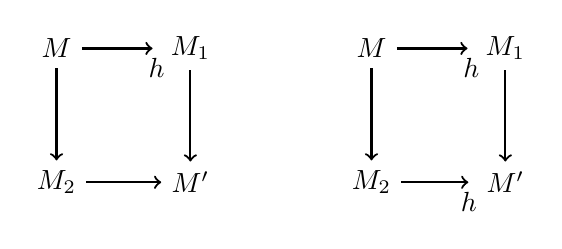
\begin{tikzpicture}[thick,node distance=17mm]
    \node (M) {$M$};
    \node (M1) [right of=M] {$M_1$};
    \node (M2) [below of=M] {$M_2$};
    \node (M') [below of=M1] {$M'$};
    \draw [->,shorten >= 1mm] (M) -- (M1) node [pos=.95,below] {$h$};
    \draw [->] (M) -- (M2); 
    \draw [->] (M2) -- (M') node [midway,above] {$\varnothing$};
    \draw [->] (M1) -- (M') node [midway,right] {$\varnothing$};

    \begin{scope}[xshift=4cm]
    \node (M) {$M$};
    \node (M1) [right of=M] {$M_1$};
    \node (M2) [below of=M] {$M_2$};
    \node (M') [below of=M1] {$M'$};
    \draw [->,shorten >= 1mm] (M) -- (M1) node [pos=.95,below] {$h$};
    \draw [->] (M) -- (M2); 
    \draw [->,shorten >= 1mm] (M2) -- (M') node [pos=.9,below] {$h$};
    \draw [->] (M1) -- (M');
    \end{scope}
  \end{tikzpicture}
  \vspace{-2ex}
  \caption{Elementary diagrams for simple $\boldsymbol{M}$.}
  \vspace{-2ex}
  \label{fig:elementary:diagram:simple}
  \end{center}
  \end{figure}
  
  That is, whenever we have co-initial steps $M \hred M_1$ and $M \to M_2$
  and $M$ is a simple term,
  then either the steps cancel each other out $M_1 \equiv M_2$ (if both are the same step),
  or they can be joined by single steps $M_1 \hred M' \redi M_2$.

  As a consequence, when projecting $M \hred M'$ over a rewrite sequence $M \to^n N$
  then either $N \to^n M'' \hredi M'$ or
  there has been cancellation and $N \to^{n-1} M'' \equiv M'$.
  Every cancellation decreases the number of steps $N \to^{n-1} M''$,
  and hence there can only finitely many cancellations.
  This implies the claim that $\cbohm{M}$ is equal to $\cbohm{N}$
  modulo a finite prefix, that is, $M \crelev{=} N$.
\end{proof}

Reduction accelerates clocks, i.e., $\smred \subseteq {\crel{{\geq}}}$.
Moreover, for simple terms the clock is invariant under reduction, see Proposition~\ref{prop:simple}.
Hence if a term $M$ has a simple reduct $N$, then $N$ has the fastest clock reachable from $M$ 
modulo a finite prefix. This justifies the following convention.
\begin{convention}
  The \emph{(minimal) clock} of a $\lambda$-term $M$ with a simple reduct $N$
  is $\cbohm{N}$, the clocked BT of $N$.
\end{convention}


For simple terms we obtain the following theorem:
\begin{theorem}\label{thm:simple}
  Let $M$ and $N$ be $\lambda$-terms.
  If there exists a reduct $N'$ of $N$
  and a simple reduct $M'$ of $M$ such that
  $M' \creli{>} N'$, then $M \ne_\beta N$.
\end{theorem}
\begin{proof}
  Assume $M =_\beta N$. Then $M' = N'$ and by confluence they have a common reduct
  $M' \mred M'' \mredi N'$.
  Since $M'$ is simple, we have $M' \crelev{=} M''$ by Proposition~\ref{prop:simple}.
Hence, $M' \creli{>} N'$ implies $M'' \creli{>} N'$,
  which would contradict $M'' \crel{\le} N'$ obtained by Proposition~\ref{prop:clocks}.
\end{proof}
Theorem~\ref{thm:simple} significantly reduces 
the proof obligation in comparison to Theorem~\ref{thm:general}.
We can pick any simple reduct $M'$ of $M$,
instead of having to reason about all reducts $M'$ of $M$.
For the case that both $M$ and $N$ are simple, there is no need to look for reducts:
\begin{proposition}\label{cor:simple:simple}
  For simple terms $M$ and $N$,
  $M \creli{\ne} N$ implies $M \ne_\beta N$.
\end{proposition}
\begin{proof}
  Assume $M = N$ then $M \mred O \mredi N$ for a common reduct $O$.
  Then $M \crelev{=} O \crelev{=} N$ by Proposition~\ref{prop:simple}. 
  Hence $M \crelev{=} N$ which contradicts $M \creli{\ne} N$.
\end{proof}

\begin{example}\label{ex:boehm:seq}
  Let $n \geq 2$.
  We compute the clocks of the fpc's 
  $\fpc{n}$ of the \boehm{} sequence.
We first reduce $\fpc{n} \defeq \leftappiterate{\fpcC}{\delta}{n}$
  with $\fpcC \defeq \mylam{f}{\omega_{f}\omega_{f}}$
  and $\omega_f \defeq \mylam{x}{f(xx)}$ to a simple term:
  \begin{align*}
    \fpc{n} x
    \to \leftappiterate{\omega_\delta \, \omega_\delta}{\delta}{n-1} x
    \mred \leftappiterate{\nf{\omega_\delta} \, \nf{\omega_\delta}}{\delta}{n-1} x
  \end{align*}
  where $\nf{\omega_\delta} = \mylam{ab}{b(aab)}$.
  We compute the clock:
  \begin{align*}
    \leftappiterate{\nf{\omega_\delta} \, \nf{\omega_\delta}}{\delta}{n-1} x
    & \hredn{2} \leftappiterate{\delta (\nf{\omega_\delta} \, \nf{\omega_\delta} \delta)}{\delta}{n-2} x
    \\
    & \hredn{2(n-2)} \delta (\leftappiterate{\nf{\omega_\delta} \, \nf{\omega_\delta}}{\delta}{n-1}) x
    \\
    & \hredn{2} x (\leftappiterate{\nf{\omega_\delta} \, \nf{\omega_\delta}}{\delta}{n-1} x) 
  \end{align*}
  We find 
  $\cbohm{\leftappiterate{\nf{\omega_\delta} \, \nf{\omega_\delta}}{\delta}{n-1} x} 
   = \annotate{2n}{(x \cbohm{\leftappiterate{\nf{\omega_\delta} \, \nf{\omega_\delta}}{\delta}{n-1} x})}$.
  Hence, for $n \geq 2$ the clock of $\fpc{n}$ is $2n$.
\end{example}
\noindent
By Theorem~\ref{thm:simple}, Example~\ref{ex:boehm:seq}
and Figure~\ref{fig:boem:y0:y1} we obtain an alternative 
proof for Theorem~\ref{thm:boehm:seq}: the \boehm{} sequence contains no duplicates.

\begin{example}\label{ex:scott:seq}
  Let $n \geq 2$.
  We compute the clocks of the fpc's 
  $U_n \defeq \leftappiterate{BY}{S}{n} I$
  of the Scott sequence; so where $Y = \fpcC$.
  We first reduce $U_n$ to a simple term:
  \begin{align*}
    U_n x 
    & \mred \leftappiterate{Y (S S)}{S}{(n-2)} I x \\
    & \to \leftappiterate{\omega_{SS}\,\omega_{SS}}{S}{(n-2)} I x \\
    & \mred \leftappiterate{\nf{\omega_{SS}}\,\nf{\omega_{SS}}}{S}{(n-2)} I x
  \end{align*}
  where $\nf{\omega_{SS}} = \mylam{abc}{bc(aabc)}$.
  We abbreviate $\theta \equiv \nf{\omega_{SS}}$.
  Then we compute the clocks for $n = 2$, $n = 3$, and $n > 3$:
  \begin{align*}
    \theta\theta I x 
    & \hredn{3} I x (\theta\theta I x) 
    \hredn{1} x (\theta\theta I x) 
    \\
    \theta\theta S I x 
    & \hredn{3} {S I(\theta\theta S I)} x
    \hredn{4} {x (\theta\theta S I x)} 
    \\
    \leftappiterate{\theta\theta}{S}{(n-2)} I x
    &\hredn{3} \leftappiterate{ S S (\theta\theta S S)}{S}{(n-4)} I x
    \\
    &\hredn{3(n-4)} S S (\leftappiterate{ \theta \theta S S }{S}{(n-4)}) I x
    \\
    &\hredn{3} S I (\leftappiterate{ \theta \theta }{S}{(n-2)} I) x
    \\
    &\hredn{4} x (\leftappiterate{ \theta \theta }{S}{(n-2)} I x)
  \end{align*}
  respectively.
  For all three cases, we find: \[\cbohm{\leftappiterate{\theta\theta}{S}{(n-2)} I x} 
   = \annotate{3(n-2)}{(x \cbohm{\leftappiterate{ \theta \theta }{S}{(n-2)} I x})}\]
\end{example}
\noindent
Using Theorem~\ref{thm:simple} we infer from Example~\ref{ex:scott:seq}
and Figure~\ref{fig:boem:y0:y1} (recall that $U_0 \conv Y_0$ and $U_1 \conv Y_1$):
\begin{corollary}
  The Scott sequence contains no duplicates.  
\end{corollary}

Plotkin~\cite{plot:2007} asked:
Is there an fpc $Y$ such that
\begin{align*}
  A_Y \equiv Y(\mylam{z}{fzz}) \conv Y(\mylam{x}{Y(\mylam{y}{fxy})}) \equiv B_Y 
\end{align*}
or in other notation: $\mymu{z}{fzz} \conv \mymu{z}{fzz}$,
where 
$\mymu{x}{M(x)} = Y(\mylam{x}{M(x)})$.
The terms $A_Y$ and $B_Y$ have the same \boehm{} tree,
which is the solution of $T = f T T$.

The terms $A_Y$ and $B_Y$ are not simple.
An extension of our clock method can be given 
which restricts the clock comparison to single paths in the clocked \boehm{} tree
along which there is no duplication of redexes.
We leave this extension to future work.
Using this extension would allow us to settle 
the question in the negative for all simple fpc's.
For Turing's fpc $\fpcT$ this is seen by computing 
the clocked BT's of $A_{\fpcT}$ and $B_{\fpcT}$.
Recall $\fpcT \equiv \eta\eta$ with $\eta \equiv \mylam{xf}{f(xxf)}$.
\begin{align*}
  A_{\fpcT} 
  &\equiv \eta\eta(\mylam{z}{fzz})
  \hredn{2} (\mylam{z}{fzz}) A_{\fpcT} \\
  & \hredn{1} f A_{\fpcT} A_{\fpcT} \\
  B_{\fpcT} 
  &\equiv \eta\eta(\mylam{x}{\eta\eta(\mylam{y}{fxy})})
  \\
  &\hredn{2} 
  (\mylam{x}{\eta\eta(\mylam{y}{fxy})}) B_{\fpcT} \\
  &\hredn{1} 
  \eta\eta(\mylam{y}{f B_{\fpcT} y})
  \\
  &\hredn{2}
  (\mylam{y}{f B_{\fpcT} y})(\eta\eta(\mylam{y}{f B_{\fpcT} y}))
  \\
  &\hredn{1}
  f B_{\fpcT} (\eta\eta(\mylam{y}{f B_{\fpcT} y}))
\end{align*}
Note that for $B_{\fpcT}$ developing the left branch takes six steps,
whereas the right only needs three.
The clocked BT's for $A_{\fpcT}$ and $B_{\fpcT}$ are depicted in Figure~\ref{fig:plotkin}
using hnf-notation (see~\cite{bare:1984} or~\cite{bare:klop:2009}).

\begin{figure}[ht!]
\begin{center}
  \begin{tikzpicture}[level distance=7mm,inner sep=0.5mm,
                      level 1/.style={sibling distance=18mm},
                      level 2/.style={sibling distance=9mm},
                      level 3/.style={sibling distance=4.5mm},
                      level 4/.style={sibling distance=2.25mm}
                     ]
    \node  {$f$} \annotatednode{$f$}{3}
      child { node {$f$} \annotatednode{$f$}{3}
        child { node {$f$} \annotatednode{$f$}{3}
          child { node {$\ldots$} }
          child { node {$\ldots$} }
        }
        child { node {$f$} \annotatednode{$f$}{3}
          child { node {$\ldots$} }
          child { node {$\ldots$} }
        }
}
      child { node {$f$} \annotatednode{$f$}{3}
        child { node {$f$} \annotatednode{$f$}{3}
          child { node {$\ldots$} }
          child { node {$\ldots$} }
        }
        child { node {$f$} \annotatednode{$f$}{3}
          child { node {$\ldots$} }
          child { node {$\ldots$} }
        }
      };
  \end{tikzpicture}\quad
  \begin{tikzpicture}[level distance=7mm,inner sep=0.5mm,
                      level 1/.style={sibling distance=18mm},
                      level 2/.style={sibling distance=9mm},
                      level 3/.style={sibling distance=4.5mm},
                      level 4/.style={sibling distance=2.25mm}
                     ]
    \node  {$f$} \annotatednode{$f$}{6}
      child { node {$f$} \annotatednode{$f$}{6}
        child { node {$f$} \annotatednode{$f$}{6}
          child { node {$\ldots$} }
          child { node {$\ldots$} }
        }
        child { node {$f$} \annotatednode{$f$}{3}
          child { node {$\ldots$} }
          child { node {$\ldots$} }
        }
}
      child { node {$f$} \annotatednode{$f$}{3}
        child { node {$f$} \annotatednode{$f$}{6}
          child { node {$\ldots$} }
          child { node {$\ldots$} }
        }
        child { node {$f$} \annotatednode{$f$}{3}
          child { node {$\ldots$} }
          child { node {$\ldots$} }
        }
      };
  \end{tikzpicture}
\caption{Clocked BT's for $\boldsymbol{A_{\fpcT}}$ and $\boldsymbol{B_{\fpcT}}$.}
\label{fig:plotkin}
\end{center}
\end{figure}

We conjecture that for no fpc $Y$, $A_Y \conv B_Y$;
maybe this requires an extension of the proof in~\cite{intri:1997}.


